\documentclass{article}
\usepackage[utf8]{inputenc}
\usepackage{placeins}
\usepackage{graphicx}
\graphicspath{ {./img/} }

\title{Relazione Progetto Programmazione}
\author{Emanuele Pischetola}
\date{December 2022}

\begin{document}

\maketitle

\section{Divisione dei ruoli}
% Stampa a schermo e degli oggetti di gioco: piske
% Gestione della fisica: saad
% Gestione della della mappa: diego
I ruoli sono stati suddivisi in base al carico di lavoro.
La suddivisione è avvenuta nel seguente modo:
\begin{itemize}
\item \textbf{Schermo} (Emanuele Pischetola): si occupa di gestire la stampa sul terminale attraverso la librerie curses/ncurses.h.
\item \textbf{Entità e Oggetti} (Emanuele Pischetola): si tratta delle classi che descrivono tutti gli elementi rappresentabili nel gioco. Sono state realizzate tramite l'uso di eriditarietà
\item \textbf{Fisica di gioco} (Saad): in generale si occupa di prendere in input lo stato di gioco corrente e restituire il nuvo stato di gioco, in base a ciò che è avvenuto.
\item \textbf{Mappa} (Diego Ammirabile): definisce la mappa corrente e di conseguenza si occupa di memorizzare le stanze visitate e il loro contenuto
\item \textbf{Game Loop} (Diego Ammirabile): % non so cosa scrivere(forse "è il main"?)
\end{itemize}

\subsection{Schermo}
Lo schermo è implementato nei file Screen.hpp, GameInterface.hpp, GameMenu.hpp, GameControls.hpp. La classe Screen è generica, mentre le altre rappresentano una specifica finestra.
\subsection{Entità e Oggetti}
Le entità di gioco sono tutte figle della classe Core, che rappresenta l'elemento più generico possibile. Le classi direttamente figlie sono Entity ovvero gli elementi "vivi".
ItemOnGround cioè gli oggetti, e Wall i muri. I file sono Core.hpp, ItemOnGround.hpp, Entity.hpp, Wall.hpp, Bullet.hpp, Player.hpp, Hostile.hpp

Mentre gli oggetti sono i figli della classe Item, che possono essere Consumabili come pozioni e chiavi, oppure dei potenziamenti alle statistiche come attacco e vita. Sono tutte implementate nel file Equipment.hpp

% inserire qui schema delle classi
\begin{figure}[!ht]
    \centering
    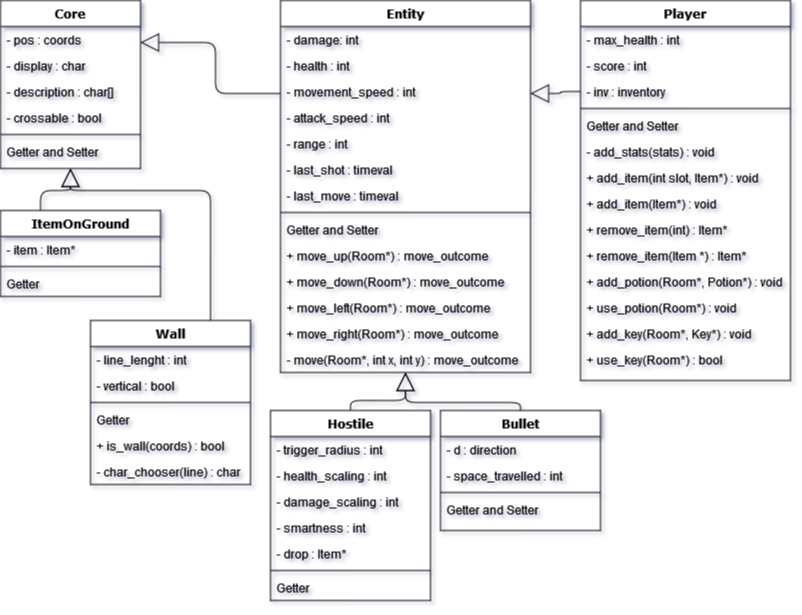
\includegraphics[width=1\textwidth]{UML_Prog_Programmazione.png}
    \caption{UML delle entità di gioco}
    \label{fig:1}
\end{figure}
\FloatBarrier

\subsection{Fisica di gioco}
I metodi della fisica di gioco sono raccolti nei file physics.h/physics.cpp, % geometry.h lo metto qui come fatto da saad?

\subsection{Mappa}
La mappa e i relativi metodi sono descritti nel file Map.h, ed è stata implementata tramite una struttura. Mentre la stanza è una classe implementata in Room.hpp. Inoltre per realizzare la mappa sono state implementate due strutture dati: la lista e la coda. Sono nei file List.hpp e Queue.hpp

\subsection{Altro}
Altri file che non ho menzionato sono constants.h che contiene tutti i valori costanti e alcune strutture, time\_handle.h che ha alcune funzioni utili per calcolare il tempo in millisecondi, questi file sono di responsabilità di E. Pischetola. Mentre gli eventi, nei file RoomEvent.hpp e Events.hpp, sono di responsabilità di D. Ammirabile.

\section{Scelte implementative}
% Organizzazione del progetto in 3 componenti comunicanti
% utilizzo degli eventi per comunicare
Abbiamo pensato di implementare il progetto divendendolo in 3 componenti fondamentali: la vista, il modello e il controller.
\subsection{Modello}
Il modello è il componente che si occupa di tenere i dati del gioco. Quindi è rappresentato dalla mappa e dalle classi Room, Core, Item e le relative classi figlie.
Esso infatti viene aggiornato dal controller ogni ciclo del game loop per rispecchiare la situazione di gioco.

Esempio: quandi il giocatore preme w per muoversi verso l'alto le coordinate dell'oggetto player vengono cambiate.
\subsection{Vista}
La vista è il componente che si occupa esclusivamente della visualizzazione grafica sul terminale, ed è rappresentato dalle classi Screen, GameMenu, GameInterface, GameOptions. 
Il compito di queste classi è infatti leggere la versione più aggiornata del modello, quindi l'oggetto di tipo Room relativo alla stanza corrente, e stampare sul terminale la corrispondente rappresentazione grafica.

Esempio: la vista vede che le coordinate del player sono cambiate, quindi cancella il carattere del player nella posizione precedente, e poi stampa il carattere del player nelle nuove coordinate.
\subsection{Controller}
Il controller si occupa di modificare il modello, è rappresentato da physics.h. I suoi metodi vengono invocati dalle altre classi.
\subsection{Eventi}
Per gestire la comunicazione tra i componenti abbiamo implementato gli eventi. Ogni volta che il controller cambia qualcosa nel modello aggiunge il relativo evento in una coda. La coda è legata alla stanza corrente, infatti è un paramentro della classe Room. Quando la stampa della vista viene invocata, essa legge la coda degli eventi ed esegue la routine associata ad ogni evento che trova.
Gli eventi si possono trovare nel file Events.hpp

\end{document}